% !TEX root = ../Dokumentation.tex
\subsection{Halterungen}
\begin{figure}[H]
\centering
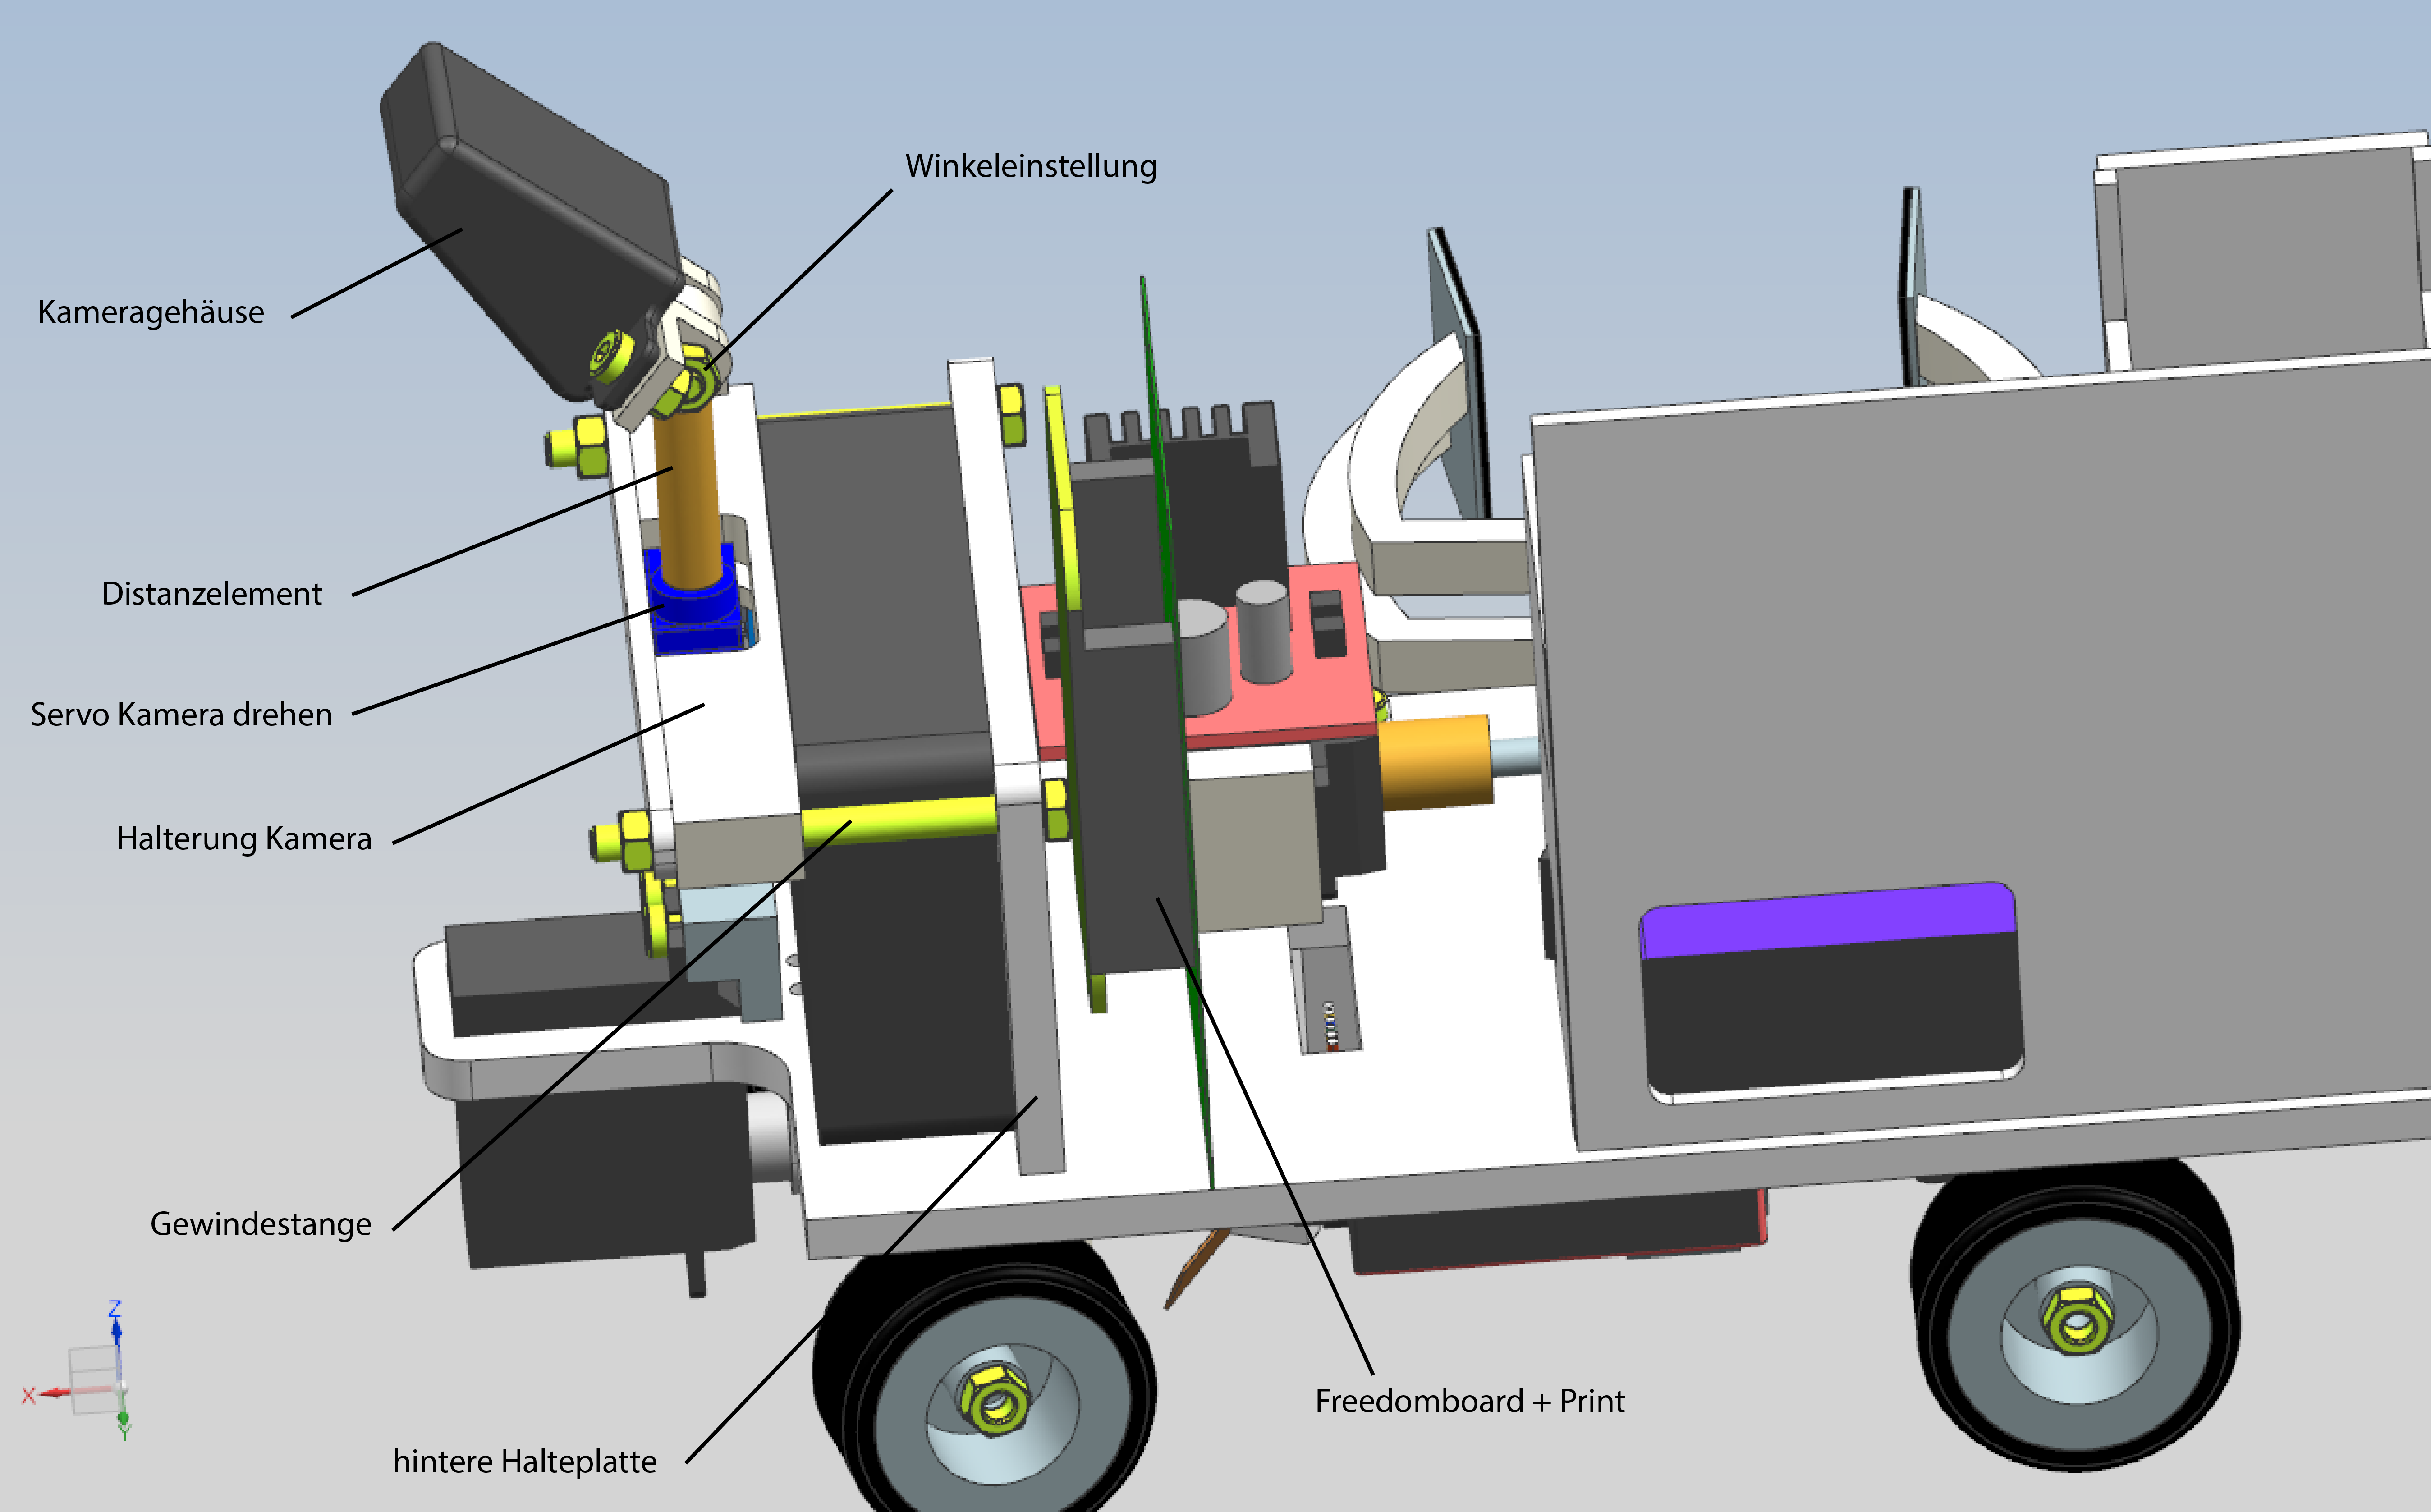
\includegraphics[width=1\textwidth]{03_Loesungskonzept/pictures/halterungen2.png}
\caption{Halterungen für Kamera, Rasperry Pi, Freedom Board und Print}
\end{figure}
\textbf{Halterung Kamera}\\[0.2cm]
Die Kamera ist auf einer festen Höhen montiert. Der Winkel zur Fahrbahn ist einstellbar. Nach Tests wurde der Winkel definitiv bestimmt und eingestellt.\\[0.2cm]
Die Kamera ist über ein Distanzelement auf dem Servo Motor montiert. Damit kann die Kamera in der Kurve gedreht werden. Der Servo Motor wird auf die Halterung (3D Druckteil) geschraubt.\\[0.2cm]
\textbf{Befestigung Rasperry Pi}\\[0.2cm]
Das Rasperry wird bei der Montage an die hintere Halteplatte gedrückt, die aus Acrylglas gefertigt ist und auf der Grundplatte angeschraubt ist. Auf der vorderen Seite wird ein 3D Druckteil und ein Acrylglasteil angebracht. Die beiden Seiten werden mit durchgehender Gewindestangen verschraubt. Dabei muss darauf geachtet werden, dass nicht zu stark angezogen wird um keine Teile zu beschädigen.\\[0.2cm]
\textbf{Befestigung Freedom Board und Print}\\[0.2cm]
Der Print und das Freedom Board wurden mit Klettverschluss auf der hinteren Halterungen des Rasperry PIs befestigt.\\[0.2cm]
\begin{figure}[H]
\centering
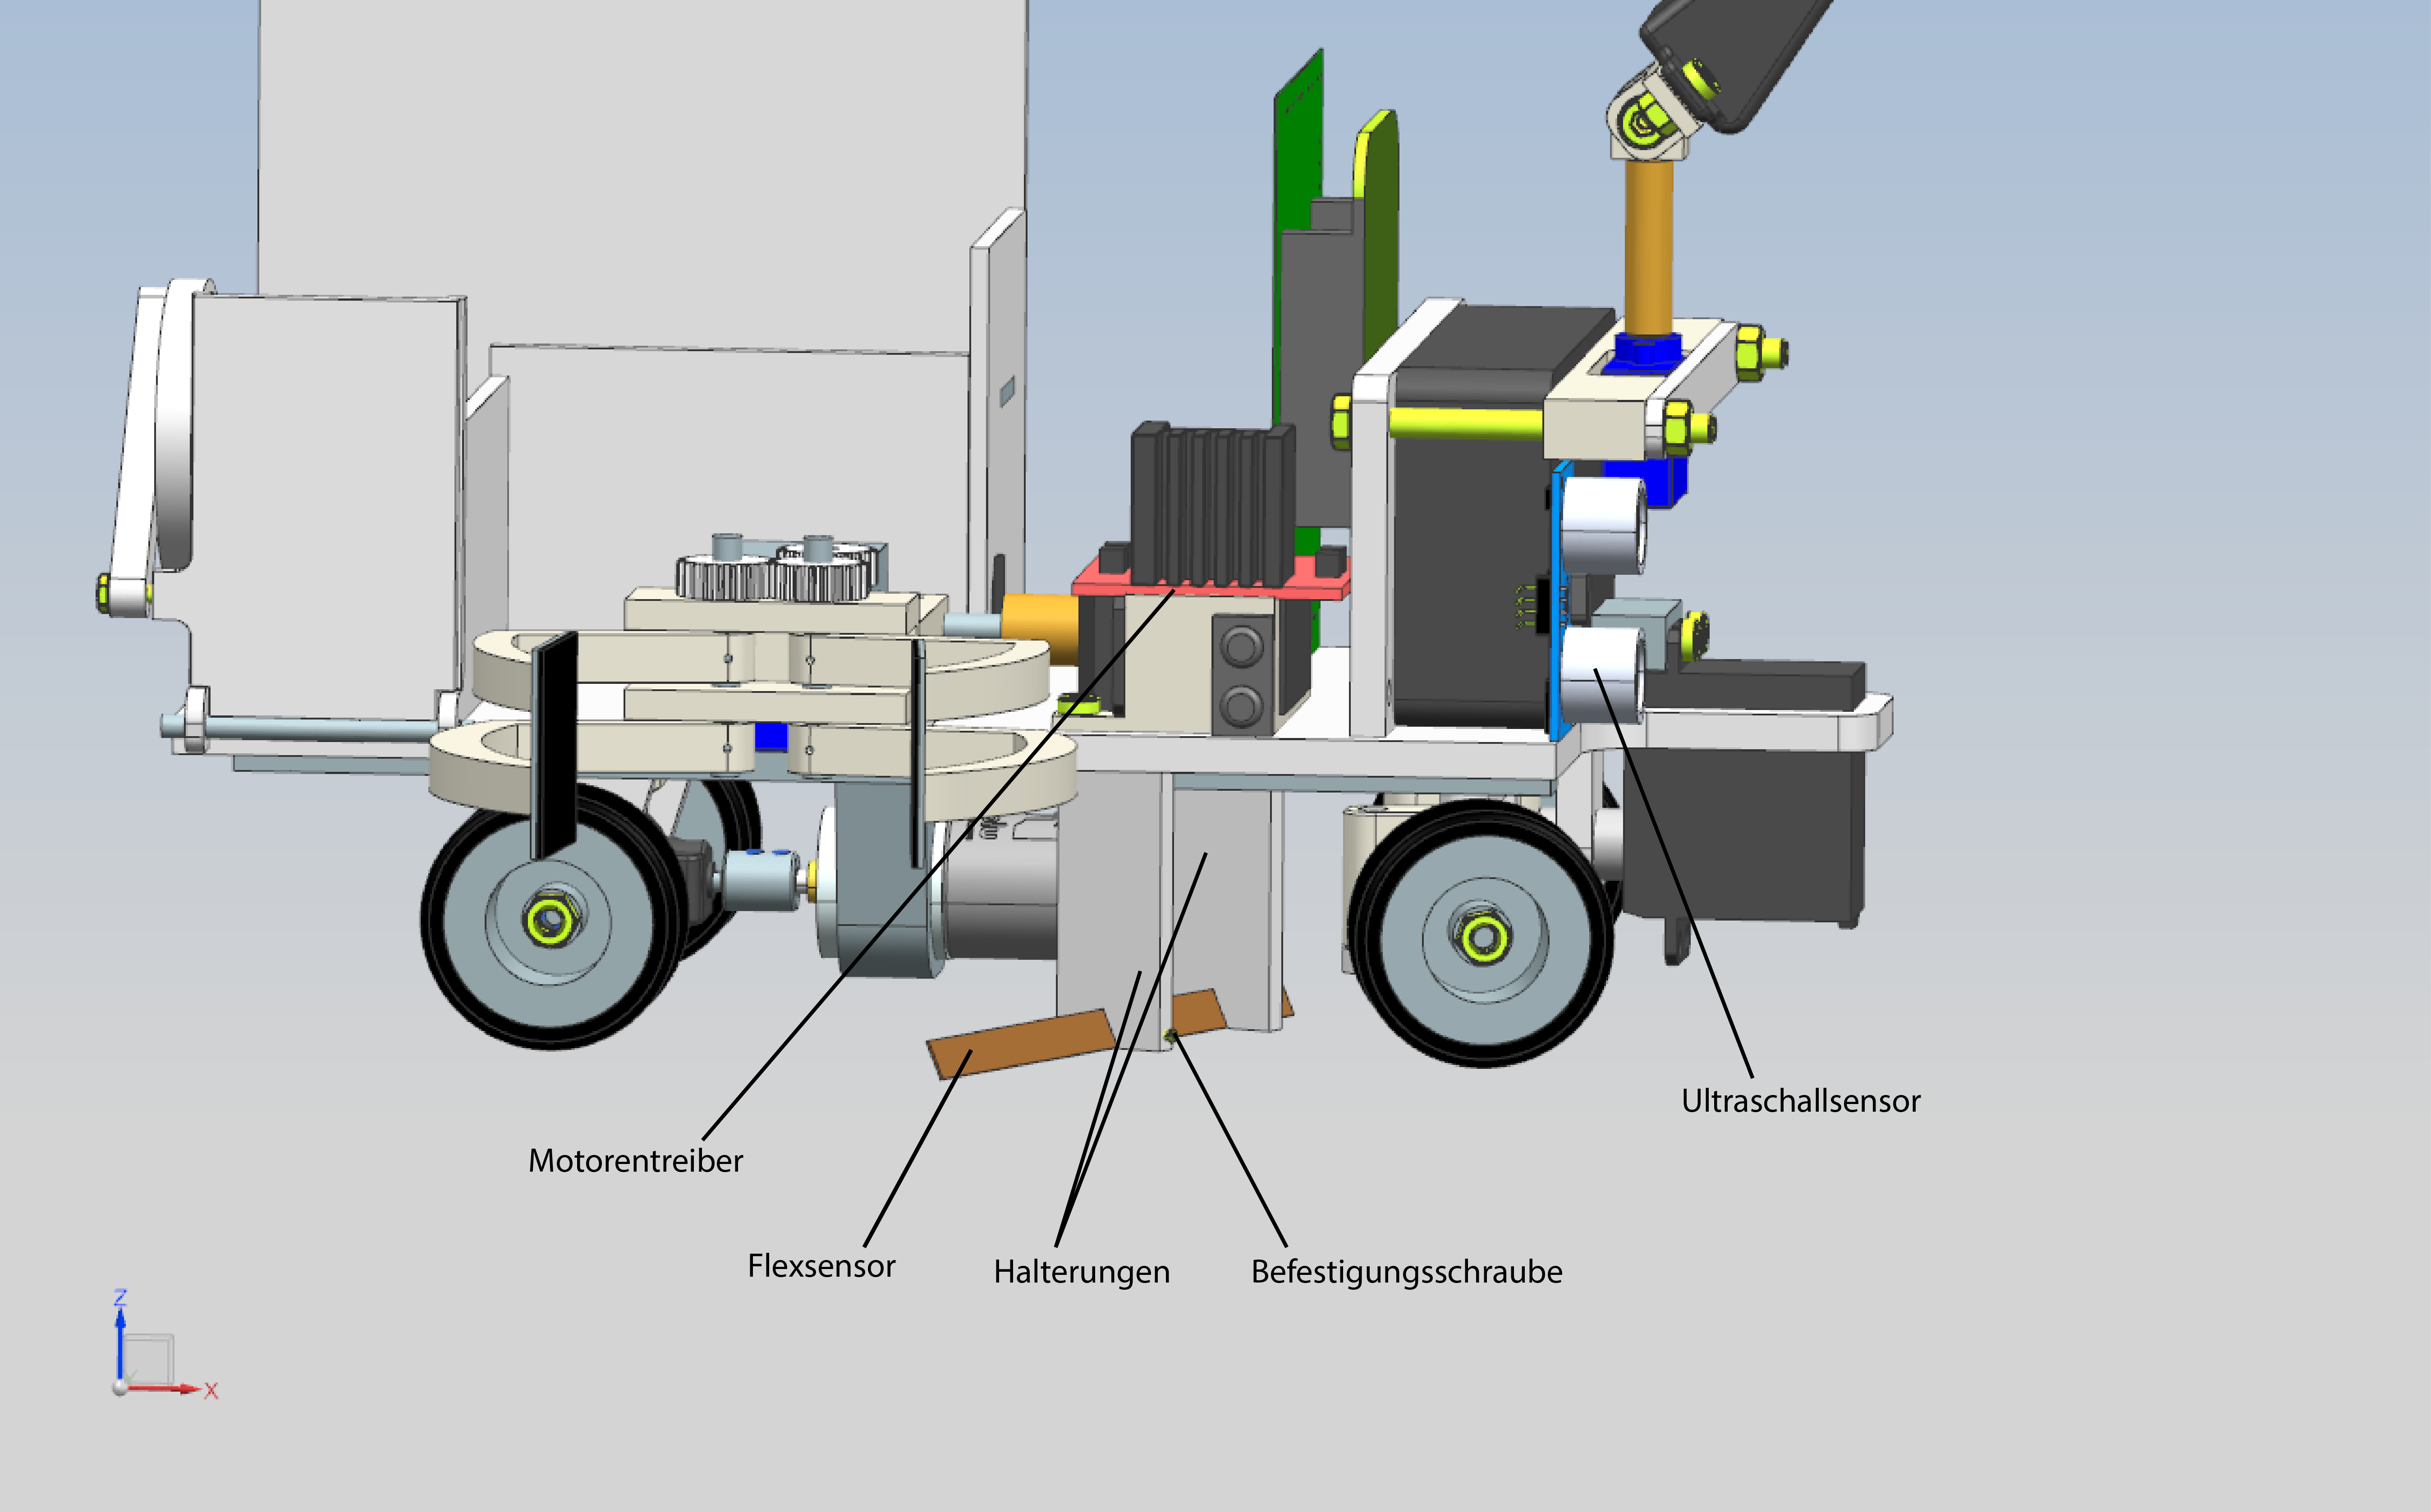
\includegraphics[width=1\textwidth]{03_Loesungskonzept/pictures/halterungen1.png}
\caption{Halterungen für Motorentreiber, Infrarotsensor und Flexsensor}
\end{figure}
\textbf{Befestigung Motorentreiber, Ultraschallsensor}\\[0.2cm]
Der Motorentreiber wurde mit Klettverschluss auf der Halterung für den Greifer drehen befestigt.\\[0.2cm]
Der Ultraschallsensor wird vorne rechts angeklettet.\\[0.2cm]
\textbf{Befestigung Flexsensor}\\[0.2cm]
Der Flexsensor wird unterhalb der Grundplatte montiert. Die zwei Halterungen wurden aus Acrylglas gelasert und unter die Grundplatte geleimt. Dabei sind die Halterungen leicht schräg. Der Flexsensor wird in die beiden Schlitze der Halterungen eingeführt. Um immer die gleiche Länge zu haben, kann der Flexsensor mit einer Schraube befestigt werden.\\[0.2cm]
\textbf{Befestigung Infrarot Sensor}\\[0.2cm]
Der Infrarot Sensor wurde auf der rechten Seite des Fahrzeugs auf die Halterung des Motors (Greifer drehen) angeklettet.